\documentclass[landscape]{article}
\usepackage[a4paper,margin=3mm,landscape]{geometry}
\usepackage[scaled=0.92]{helvet}
\usepackage{multicol, multirow}
\usepackage{makecell}
\usepackage{array} 
\usepackage[table]{xcolor}
\usepackage{enumitem} 
\usepackage{amssymb}
\usepackage{graphicx}
\setlist{nosep}

\graphicspath{{./images/}}

\pdfinfo{
    /Title (CS2106 Cheatsheet.pdf)
    /Creator (TeX)
    /Producer (pdfTeX 1.40.0)
    /Author (Selwyn Ang)
    /Subject (CS2106)
    /Keywords (CS2106, Cheatsheet, NUS, Introduction to Operating Systems) 
}

% Turn off header and footer
\pagestyle{empty}


\makeatletter
\DeclareRobustCommand\smaller{\@setfontsize\smaller{6pt}{6.5pt}}
\makeatother

% redefine section commands to use less space
\makeatletter
\renewcommand{\section}{\@startsection{section}{1}{0mm}%
  {-0.1ex plus -0.1ex minus -0.1ex}%
  {0.1ex plus .1ex minus 0.1ex}%
{\normalfont\small\bfseries}}
\renewcommand{\subsection}{\@startsection{subsection}{2}{0mm}%
  {-0.1ex plus -0.1ex minus -0.1ex}%
  {0.1ex plus .1ex minus 0.1ex}%
{\normalfont\scriptsize\bfseries}}
\renewcommand{\subsubsection}{\@startsection{subsubsection}{3}{0mm}%
  {-0.1ex plus -0.1ex minus -0.1ex}%
  {0.1ex plus .1ex minus 0.1ex}%
{\normalfont\smaller\bfseries}}%
\makeatother



\renewcommand{\familydefault}{\sfdefault}
\renewcommand\rmdefault{\sfdefault}
%  makes nested numbering (e.g. 1.1.1, 1.1.2, etc)
\renewcommand{\labelenumii}{\theenumii}
\renewcommand{\theenumii}{\theenumi.\arabic{enumii}.}
\renewcommand\labelitemii{•}
\renewcommand\labelitemiii{•}

\setlength{\parindent}{0pt}
\setlength{\parskip}{0pt plus 0.5ex}
\setlength{\columnsep}{0.2cm}
%% adjust spacing for all itemize/enumerate
\setlength{\leftmargini}{0.5cm}
\setlength{\leftmarginii}{0.5cm}
\setlist[itemize,1]{leftmargin=2mm,labelindent=1mm,labelsep=1mm}
\setlist[itemize,2]{leftmargin=2mm,labelindent=1mm,labelsep=1mm}
\setlist[itemize,3]{leftmargin=2mm,labelindent=1mm,labelsep=1mm}
\setlist[enumerate,1]{leftmargin=2mm,labelindent=1mm,labelsep=1mm}
\setlist[enumerate,2]{leftmargin=2mm,labelindent=1mm,labelsep=1mm}
\setlist[enumerate,3]{leftmargin=2mm,labelindent=1mm,labelsep=1mm}

% tightcenter
\newenvironment{tightcenter}{%
  \setlength\topsep{0pt}
  \setlength\parskip{0pt}
  \begin{center}
    }{%
  \end{center}
}

% boxed
\newenvironment{tightbox}{%
  \setlength\topsep{0pt}
  \setlength\parskip{0pt}
  \begin{center}
    \begin{tabular}{|@{\hspace{\dimexpr\fboxsep+0.5\arrayrulewidth}}c@{\hspace{\dimexpr\fboxsep+0.5\arrayrulewidth}}|}
      \hline
    }
    {%
    \\ \hline
    \end{tabular}
  \end{center}
}

% fixed width box
\newenvironment{fixedbox}[1][0.7]{
  \setlength\topsep{0pt}
  \setlength\parskip{0pt}
  \begin{center}
    \begin{tabular}{|>{\centering\arraybackslash}m{#1\linewidth}|}
    \hline
  }{
  \\ \hline
  \end{tabular}
  \end{center}
}

% definition of a new term
\usepackage{soul}
\definecolor{paleyellow}{RGB}{251,243,218}
\newcommand{\definition}[2][]{\sethlcolor{paleyellow}\hl{\textbf{#2}} #1  $\rightarrow$}
% inline definition
\newcommand{\ildefinition}[1]{\sethlcolor{paleyellow}\hl{\textbf{#1}}}

% important note (attention)
\newcommand{\attention}{{\color{red}\textbf{! }}}

% nice proof
\newenvironment{niceproof}[1][Proof]
{%
  \sbox0{\textit{#1}. }%
  \list{}{\labelwidth\wd0 \leftmargin\wd0 \labelsep 0pt }
\item[\usebox0]}
  {\endlist}


\usepackage{color, soul}
\usepackage{listings}
\usepackage{inconsolata}

\definecolor{codegreen}{rgb}{0,0.6,0}
\definecolor{codegray}{rgb}{0.5,0.5,0.5}
\definecolor{codepurple}{HTML}{C42043}
\definecolor{backcolour}{HTML}{F2F2F2}
\definecolor{bookColor}{cmyk}{0,0,0,0.90}

\newcommand{\code}[1]{\texttt{\sethlcolor{backcolour}\hl{$\,$#1$\,$}}}

% SQL code blocks
% define SQL styles
\lstdefinestyle{mySQL}{%
  language=SQL,
  backgroundcolor=\color{backcolour},
  commentstyle=\color{codegreen},
  keywordstyle=\color{codepurple},
  numberstyle=\numberstyle,
  stringstyle=\color{codepurple},
  basicstyle=\scriptsize\ttfamily,
  breaklines=true,
}



% --------------------------------------------------------

\begin{document}
\raggedright
\tiny
\begin{multicols*}{6}
    \setlength{\columnseprule}{0.25pt}

    \begin{tightcenter}
        \fbox{%
          \parbox{0.8\linewidth}{\centering \textcolor{black}{
              {\Large\textbf{CS2106 Finals}}
            \\ \normalsize{AY23/24 SEM 2}}
            \\ {\footnotesize \textcolor{gray}{github/SelwynAng}}
          }%
        }
    \end{tightcenter}
    
    \section{Synchronisation}
    \subsection{Race Conditions}
    \begin{itemize}
      \item Happens when execution of concurrent processes is non-deterministic
      \item Process which reaches the end first is the one that loses
      \item Each statement of a process consists of 
      \begin{enumerate}
        \item Load operation (Loads value from resource intro register)
        \item Register operation
        \item Store operation (Stores value from register into resource)
      \end{enumerate}
      \item Bad behavior occurs when different processes interleave
      \item \underline{No. of inter-leavings} = (nm!)/(m!)\textsuperscript{n} where there are \verb|n| threads, \verb|m| instructions per thread
    \end{itemize}
    
    \subsection{Critical Section}
    \begin{itemize}
      \item \textbf{Definition of Critical Section:} Section of code that performs a read, update \& write of a shared resource (code segment with race condition) $\rightarrow$ Only 1 process can execute in Critical Section at any point of time
      \item \textbf{Properties of Correct Critical Section Implementation}
      \begin{enumerate}
        \item \underline{Mutual Exclusion:} If a process is executing in CS, all other processes are prevented from entering CS
        \item \underline{Progress:} If no process in CS, 1 of waiting processes should be granted access
        \item \underline{Bounded Wait:} After a process P\textsubscript{i} requests to enter CS, there exists an upper-bound no. of times other processes can enter CS before P\textsubscript{i}
        \item \underline{Independence:} Process not executing in CS should never block other processes
      \end{enumerate}
      \item \textbf{Symptoms of Incorrect Synchronisation}
      \begin{enumerate}
        \item \underline{Deadlock:} All processes are blocked $\rightarrow$ No Progress
        \item \underline{Livelock:} Processes keep changing state to avoid deadlock (processes are not considered blocked) $\rightarrow$ No Progress
        \item \underline{Starvation:} Some processes are blocked forever
      \end{enumerate}
    \end{itemize}

    \subsection{Assembly-level Implementation of CS}
    \begin{itemize}
      \item Mechanism provided by processor
    \end{itemize}
    \subsubsection{Test \& Set}
    \begin{itemize}
      \item \textbf{Overview:} Takes a memory address M $\rightarrow$ Returns current content at M \& Sets content of M to 1
      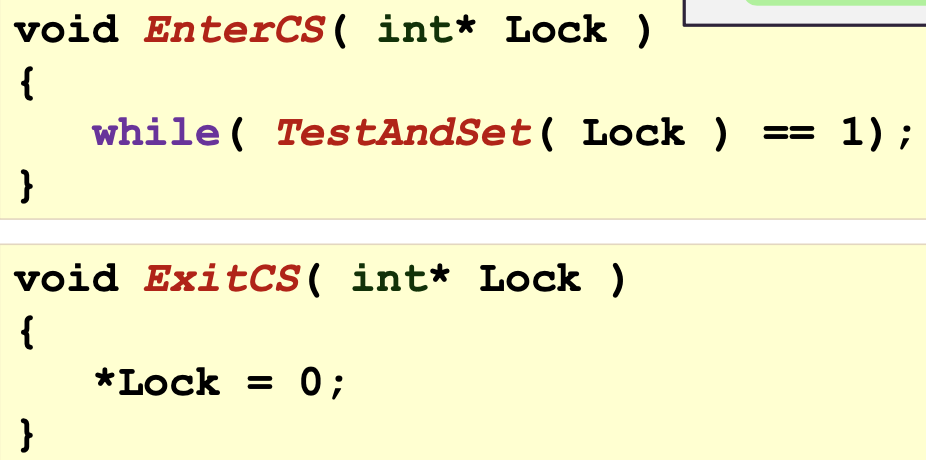
\includegraphics[width=0.75\linewidth]{1_testandset.png}
      \item \textbf{Procedure:}
      \begin{enumerate}
        \item Initially, Lock == 0 $\rightarrow$ \verb|TestAndSet(Lock)| returns 0 and sets Lock == 1
        \item While loop of 1st process exits $\rightarrow$ 1st process entered CS successfully
        \item Other processes cannot enter CS as Lock == 1 $\rightarrow$ While loops will not exit for those processes
        \item Upon exiting CS, set Lock == 0 $\rightarrow$ Other processes can enter CS
      \end{enumerate}
      \item \textbf{Cons:} Employs busy waiting for blocked processes (keeps checking while loop condition until it is safe to enter CS) $\rightarrow$ Waste of processing power
    \end{itemize}

    \subsection{High-level Language Implementation of CS}
    \begin{itemize}
      \item Utilize only normal programming constructs
      \item \textbf{Flaws of certain implementations:}
      \begin{enumerate}
        \item \underline{Preemption:} P\textsubscript{0} gets preempted after while loop $\rightarrow$ P\textsubscript{1} sees that lock == 0, exits while loop \& sets lock == 1 $\rightarrow$ P\textsubscript{1} hands control back to P\textsubscript{0} while lock == 1 \& P\textsubscript{1} is in CS $\rightarrow$ P\textsubscript{0} has checked the while loop before already \& would just enter CS (Mutual Exclusion violated)
        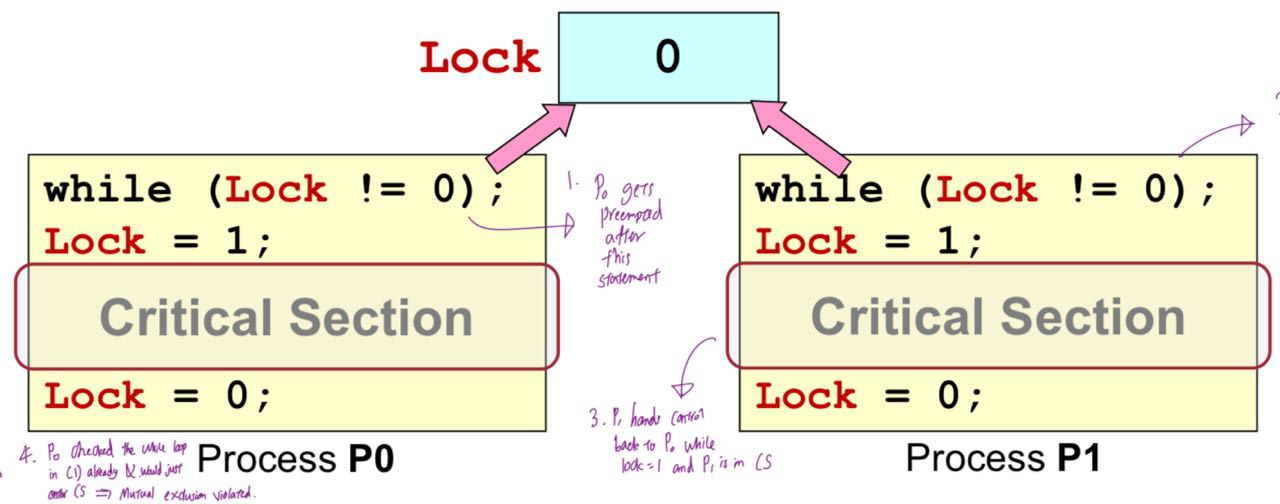
\includegraphics[width=0.9\linewidth]{2_attempt1.jpg}
        \item \underline{Disabling \& enabling interrupts:} Prevents context switch when a process is in CS (preemption requires interrupts), but \\ (1): Process crashes in CS, no way to re-enable interrupts $\rightarrow$ system shuts down; (2): Busy waiting employed; (3): Permission needed to disable/enable interrupts; (4): Ineffective on multi-CPU systems (If processes are on different CPUs, disabling a process' interrupts will only disable interrupts on its CPU, other CPU is not affected, race condition still occurs)
        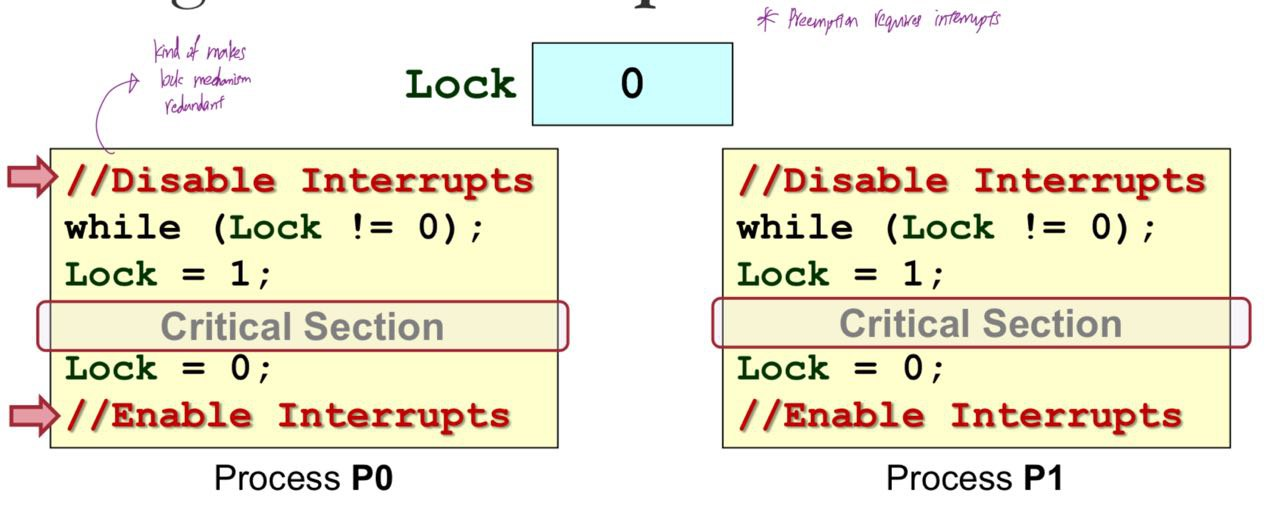
\includegraphics[width=0.9\linewidth]{3_attempt2.jpg}
        \item \underline{Failure to enter CS:} P\textsubscript{0} does not manage to enter CS, P\textsubscript{1} can starve $\rightarrow$ fufils Mutual Exclusion, but violates Independence
        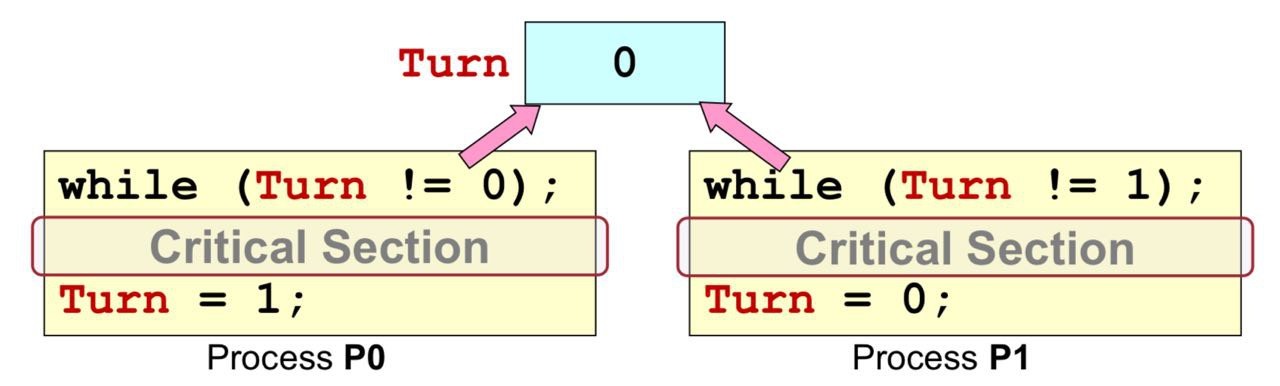
\includegraphics[width=0.9\linewidth]{4_attempt3.jpg}
        \item \underline{Deadlock:} P\textsubscript{0} sets \verb|Want[0] == 1| \& preempted $\rightarrow$ P\textsubscript{1} sets \verb|Want[1] == 1| $\rightarrow$ Both processes are stuck at while loop
        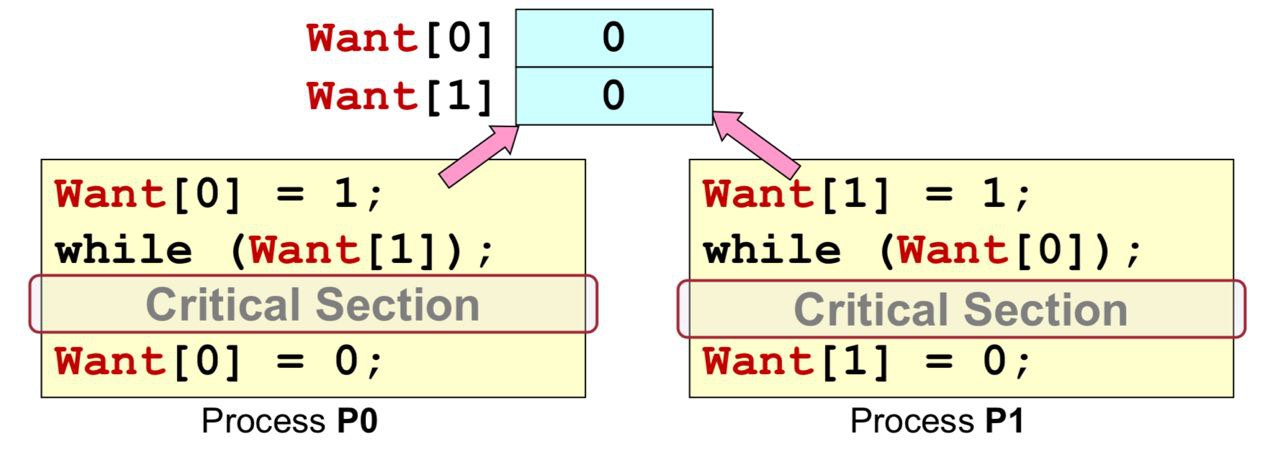
\includegraphics[width=0.9\linewidth]{5_attempt4.jpg}
      \end{enumerate}
    \end{itemize}
    \subsubsection{Peterson Algorithm}
    \begin{itemize}
      \item \textbf{Overview (Analogy of boarding bus where bus is CS):} A process will WANT to enter CS \& then gives TURN to other process $\rightarrow$ If P\textsubscript{i} gives TURN to P\textsubscript{j} but P\textsubscript{j} don't want to enter CS, P\textsubscript{i} will enter CS $\rightarrow$ Final TURN value ultimately determines which process can enter CS (only when both processes WANT to enter CS)
      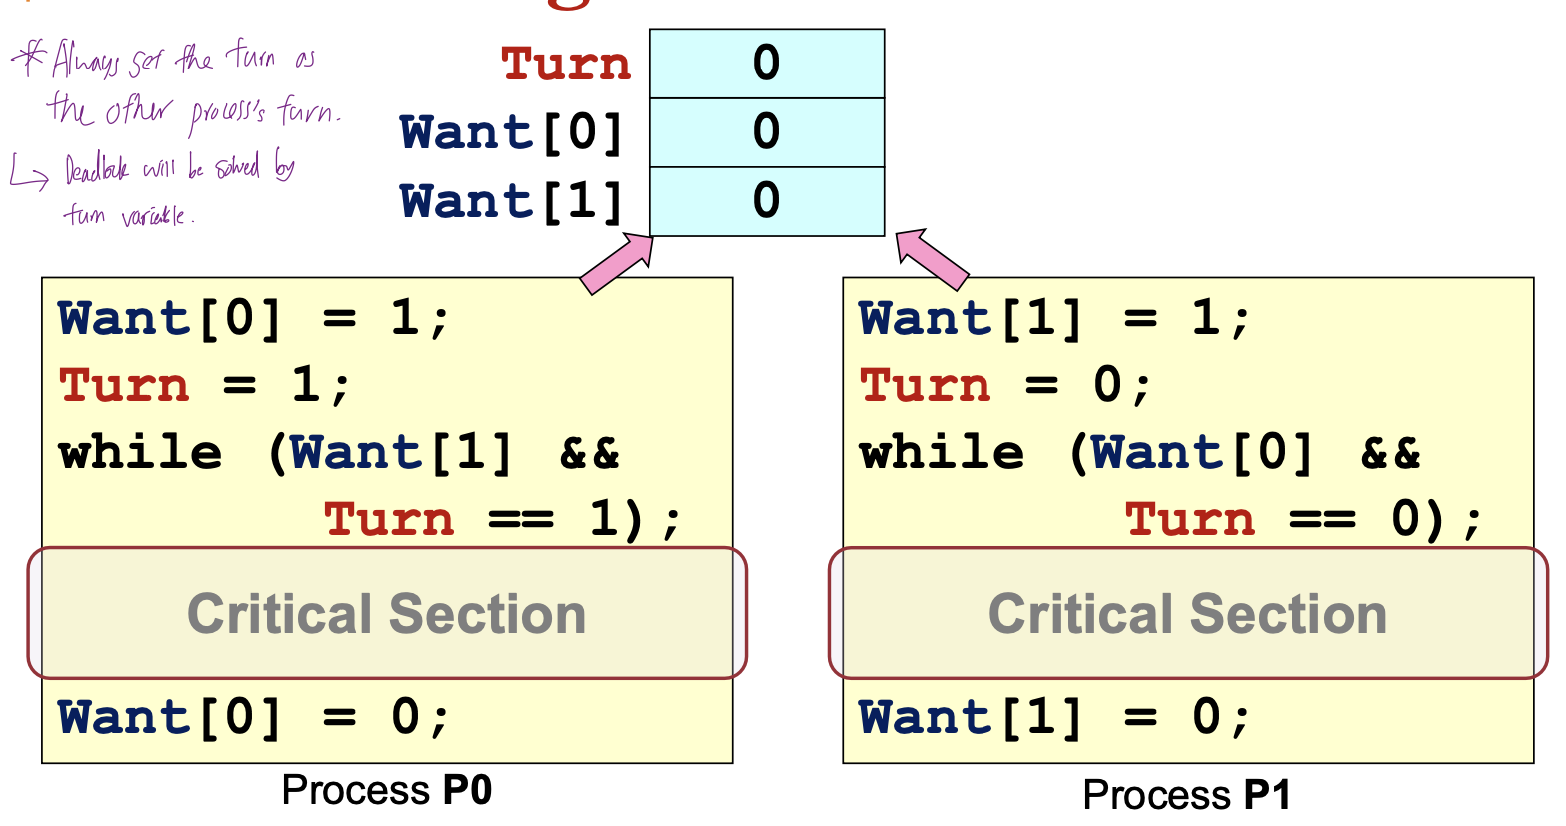
\includegraphics[width=0.9\linewidth]{6_peterson.png}
      \item \textbf{Scenarios:}
      \begin{enumerate}
        \item Both P\textsubscript{0} \& P\textsubscript{1} WANT, TURN == 0 $\rightarrow$ P\textsubscript{0} enters CS, P\textsubscript{1} blocked
        \item Both P\textsubscript{0} \& P\textsubscript{1} WANT, TURN == 1 $\rightarrow$ P\textsubscript{0} blocked, P\textsubscript{1} enters CS
        \item P\textsubscript{0} WANT \& P\textsubscript{1} don't WANT, TURN == 1 $\rightarrow$ P\textsubscript{0} enters CS, P\textsubscript{1} will get blocked even if it WANTS \& sets TURN == 0 eventually
        \item P\textsubscript{0} don't WANT \& P\textsubscript{1} WANT, TURN == 0 $\rightarrow$ P\textsubscript{1} enters CS, P\textsubscript{0} will get blocked even if it WANTS \& sets TURN == 1 eventually
      \end{enumerate}
    \end{itemize}

    \subsection{Semaphores Implementation of CS}
    \subsubsection{Semaphores}
    \begin{itemize}
      \item Provides a way to block a number of processes \& a way to unblock $\geq$ 1 sleeping process
      \item A semaphore \verb|S| contains an integer value (Initialised to any non-negative value)
      \item Given S\textsubscript{initial} $\geq$ 0, S\textsubscript{current} = S\textsubscript{initial} + No. of signal operations executed - No. of wait operations completed
      \item \textbf{Semaphore Operations:}
      \begin{enumerate}
        \item \verb|Wait(S)|: If \verb|S| $\leq$ 0, process blocks $\rightarrow$ After process unblocks, decrement \verb|S| (Code: \verb|P(Semaphore S) { while(S <= 0); S --;}|)
        \item \verb|Signal(S)|: Increment \verb|S| \& unblocks 1 blocked process if any (Signal never blocks) (Code: \verb|V(Semaphore S) {S++;}|)
      \end{enumerate}
      \item \textbf{Semaphore Types:}
      \begin{enumerate}
        \item \underline{General Semaphore:} S $\geq$ 0
        \item \underline{Binary Semaphore:} S = 0 or 1 (General semaphores can be mimicked by binary semaphores)
      \end{enumerate}
      \item \textbf{Semaphores in Critical Section:}
      \begin{itemize}
        \item Place \verb|Wait(S)| before CS \& \verb|Signal(S)| after CS $\rightarrow$ ensures mutual exclusion
        \item \underline{Binary Semaphore Implementation:}(1): S\textsubscript{initial} = 1 \& there are 2 processes P\textsubscript{0} \& P\textsubscript{1} trying to access shared resource in CS; (2): P\textsubscript{0} calls \verb|Wait(S)| $\rightarrow$ Since S = 1, it does not block \& proceeds to decrement S to 0 $\rightarrow$ P\textsubscript{0} enters CS; (3):  P\textsubscript{1} calls \verb|Wait(S)| $\rightarrow$ Since S = 0,  P\textsubscript{1} blocks \& cannot enter CS; (4):  P\textsubscript{0} finishes CS \& calls \verb|Signal(S)| $\rightarrow$ S incremented back to 1; (5):  P\textsubscript{1} becomes unblocked, S decremented back to 0, P\textsubscript{1} enters CS, calls \verb|Signal(S)| \& increments S to 1
        \item \underline{General Semaphore Implementation:} Can be generalised from binary semaphore implementation (eg. S\textsubscript{initial} = 2, 3 processes trying to access 2 shared resources in CS)
      \end{itemize}
    \end{itemize}
    \subsubsection{Proofs of Semaphore Correctness}
    \begin{enumerate}
      \item \textbf{Semaphore ensuring mutex in CS:} N\textsubscript{CS} = No. of processes in CS = \#Wait(S) - \#Signal(S) $\rightarrow$ Given S\textsubscript{initial} = 1, S\textsubscript{current} = 1 + \#Signal(S) - \#Wait(S) $\rightarrow$ S\textsubscript{current} + N\textsubscript{CS} = 1 $\rightarrow$ Since S\textsubscript{current} $\geq$ 0, hence N\textsubscript{CS} $\leq$ 1
      \item \textbf{Semaphore preventing deadlock:} Deadlock means all processes stuck at \verb|Wait(S)| $\rightarrow$ S\textsubscript{current} = 0 \& N\textsubscript{CS} = 0 $\rightarrow$ But S\textsubscript{current} + N\textsubscript{CS} = 1 (Contradiction)
      \item \textbf{Semaphore preventing starvation:} Suppose P\textsubscript{1} is blocked at \verb|Wait(S)|, P\textsubscript{2} is in CS $\rightarrow$ P\textsubscript{2} exits CS with \verb|Signal(S)| $\rightarrow$ If no other processes sleeping, P\textsubscript{1} wakes up OR If there are other processes, P\textsubscript{1} eventually wakes up (assuming fair scheduling)
    \end{enumerate}
    \subsubsection{Disadvantages of Semaphores}
    \begin{itemize}
      \item Can result in Deadlock if used incorrectly
      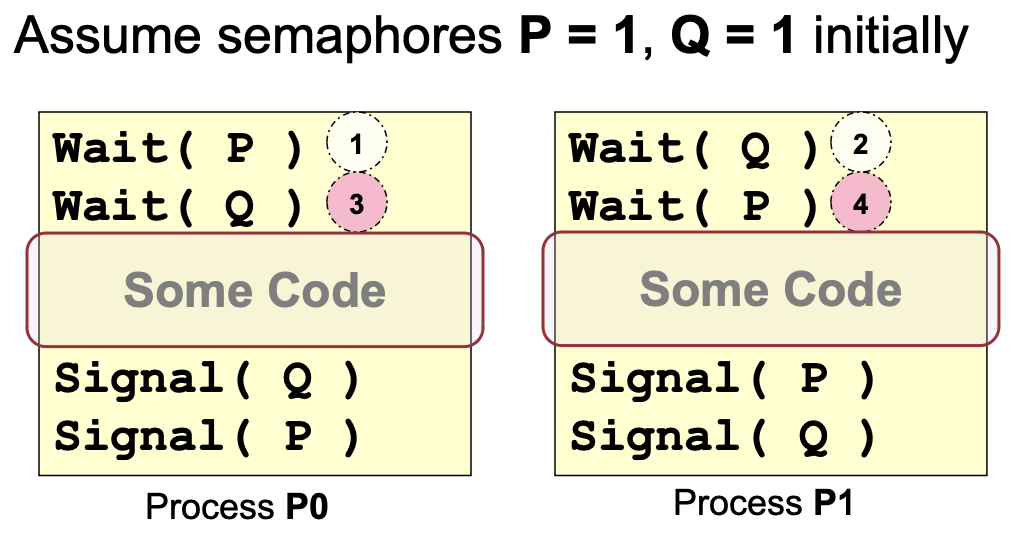
\includegraphics[width=0.75\linewidth]{7_semaphore_deadlock.png}
      \begin{enumerate}
        \item P\textsubscript{0} calls \verb|Wait(P)| \&  P\textsubscript{1} calls \verb|Wait(Q)| $\rightarrow$ P = 0 \& P = 0
        \item P\textsubscript{0} calls \verb|Wait(Q)| \&  P\textsubscript{1} calls \verb|Wait(P)| $\rightarrow$ P\textsubscript{0} \& P\textsubscript{1} both become blocked as P = 0 \& Q = 0 already
        \item P is held by P\textsubscript{0} \& Q is held by P\textsubscript{1} $\rightarrow$ Signal of both processes cannot be reached to increment the semaphores (both processes reach deadlock)
      \end{enumerate}
    \end{itemize}
    
    \subsection{Classical Synchronisation Problems}
    \subsubsection{Producer-Consumer Problem}
    \begin{itemize}
      \item \textbf{Overview:}
      \begin{itemize}
        \item Processes share a bounded buffer of size K
        \item \underline{Constraints:} (1): Producers produce items to insert into buffer only when buffer is not full; (2): Consumers remove items from buffer only when buffer is not empty; (3): Producer should not produce when another producer is producing; (4): Consumer should not remove when another consumer is removing; (5): Producer \& consumer should not produce \& consume at same time
      \end{itemize}
      \item \textbf{Naive Solution (Busy waiting):}
      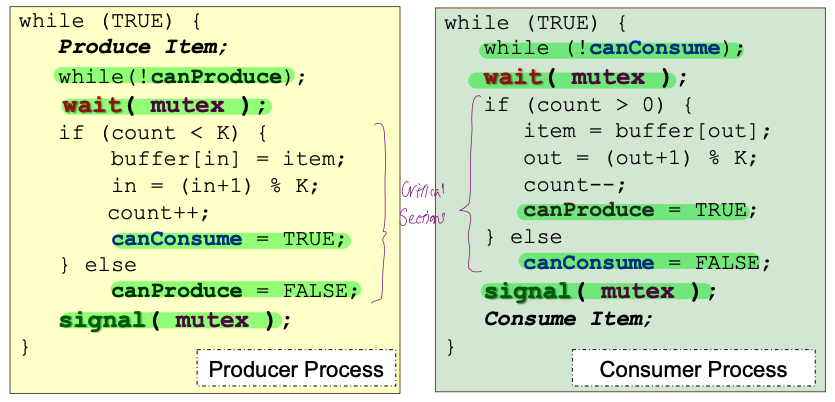
\includegraphics[width=1.0\linewidth]{8_reader_writer_naive.png}
      \begin{itemize}
        \item Initially, \verb|canProduce|=TRUE, \verb|canConsume|=FALSE, \verb|mutex|=1
        \item Correctly solves problem, but busy waiting is still used in while loop
      \end{itemize}
      \item \textbf{3 Semaphores Solution (Blocking version):}
      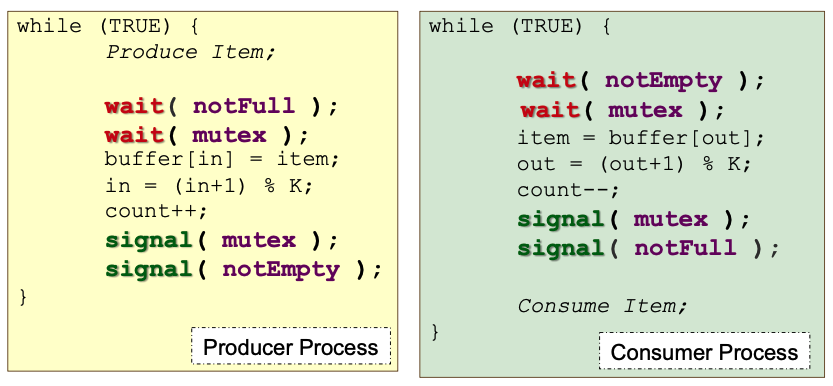
\includegraphics[width=1.0\linewidth]{9_three_sema_slon.png}
      \begin{itemize}
        \item \verb|mutex|: binary semaphore that is used to acquire \& release the lock (ensures only 1 producer/consumer in CS); \verb|notFull|: general semaphore whose initial value == K (represents no. of empty slots); \verb|notEmpty|: general semaphore whose initial value == 0 (represents no. of occupied slots)
        \item \underline{Producer perspective:} Producer calling \verb|Wait(notFull)| sees notFull \textgreater 0, indicating buffer still has space $\rightarrow$ calls \verb|Wait(mutex)| to acquire lock, inserts item, calls \verb|Signal(mutex)| to release lock $\rightarrow$ Producer calls \verb|Signal(notEmpty)| to $\uparrow$ value of \verb|notEmpty|, indicating 1 item inserted (If \verb|notFull| == 0, buffer is full \& producer is blocked until a consumer removes an item \& calls \verb|Signal(notFull)|)
        \item \underline{Consumer perspective:} Consumer calling \verb|Wait(notEmpty)| sees notEmpty \textgreater 0, indicating buffer still has items $\rightarrow$ calls \verb|Wait(mutex)| to acquire lock, removes item, calls \verb|Signal(mutex)| to release lock $\rightarrow$ Consumer calls \verb|Signal(notFull)| to $\uparrow$ value of \verb|notFull|, indicating 1 item removed (if \verb|notEmpty| == 0, buffer is empty \& consumer is blocked until a producer inserts an item \& calls \verb|Signal(notEmpty)|)
      \end{itemize}
    \end{itemize}

    \subsubsection{Reader-Writer Problem}
    \begin{itemize}
      \item \textbf{Overview:}
      \begin{itemize}
        \item Processes share a data structure where a Reader retrieves information \& a Writer modifies information
        \item \underline{Constraints:} (1): Only 1 writer can access data structure (no other writer or reader should access at same time); (2): Reader can access data structure at same time as other Readers \\
      \end{itemize}
      \item \textbf{Semaphore Solution:} \\
      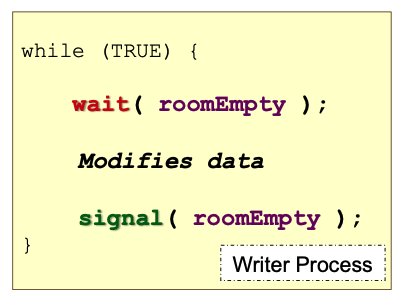
\includegraphics[width=0.45\linewidth]{10_writer.png}
      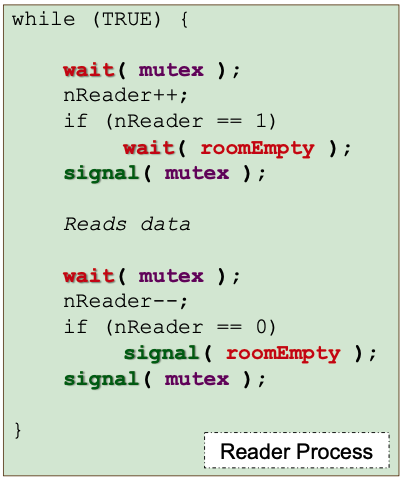
\includegraphics[width=0.5\linewidth]{11_reader.png}
      \begin{itemize}
        \item \verb|nReader|: Integer variable initialised to 0 (keeps track of current no. of readers), \verb|roomEmpty|: initialised to 1 (keeps track of presence of readers \& writers currently accessing data structure), \verb|mutex|: initialised to 1, ensure mutual exclusion when \verb|nReader| is updated (shared variable which can be updated by multiple readers)
        \item \underline{Writer perspective:} Writer calls \verb|Wait(roomEmpty)|, indicating that no other reader/writer can access data structure $\rightarrow$ Enters CS, modifies data $\rightarrow$ calls \verb|Signal(roomEmpty)|, other readers/writers can now access
        \item \underline{Reader perspective:} Reader tries to access data structure \& increments \verb|nReader| $\rightarrow$ If \verb|nReader| == 1, it means there is $\geq$ 1 reader present $\rightarrow$ Reader calls \verb|Wait(roomEmpty| which prevents writer from accessing data structure $\rightarrow$ After reader is done, \verb|nReader| is decremented $\rightarrow$ If \verb|nReader| == 0, there are no more readers present, can call \verb|Signal(roomEmpty)|, allowing writer access
        \item Reader is not bounded roomEmpty semaphores as multiple readers can access data structure at same time
        \item \underline{Potential issue:} If reader arrival rate \textgreater reader depart rate $\rightarrow$ \verb|nReader| may not be able to decrement to 0 \& just keeps increasing $\rightarrow$ writers will forever be blocked since \verb|Signal(roomEmpty)| will not be called
      \end{itemize}
    \end{itemize}

    \subsubsection{Dining Philosopher Problem}
    \begin{itemize}
      \item \textbf{Overview:} 5 philosophers are seated around a table, 5 single chopstick placed between each pair of philosophers $\rightarrow$ When any philosopher wants to eat, he has to acquire both left \& right chopsticks (Have to devise deadlock-free \& starve-free way for philosopher to eat)
      \item \textbf{Naive method:} \verb|Think(); takeChpStk(LEFT); takeChpStk(RIGHT);| \verb|Eat(); putChpStk(LEFT); putChpStk(RIGHT);| \\ All pick up left chpstk together $\rightarrow$ each philosopher cannot pick up right chpstk(Deadlock occurs \& cannot eat); Can make philosopher put down left chpstk if right chpstk cannot be acquired $\rightarrow$ Left chpstk will be taken up \& down repeatedly (livelock occurs)
      \item \textbf{Naive method with Mutex:} Surround above code with \verb|Wait(mutex)| \& \verb|Signal(mutex)| $\rightarrow$ but only 1 philosopher can take, eat, put at a time (inefficient)
      \item \textbf{Tanenbaum Solution:} \\
      \begin{multicols}{2}
        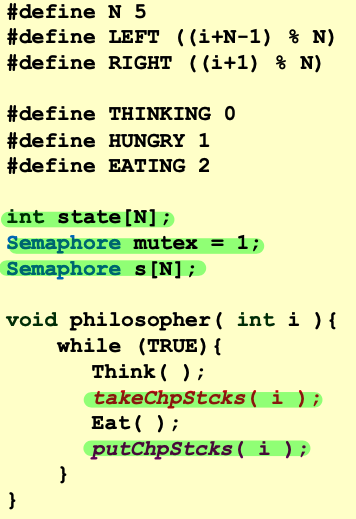
\includegraphics[width=1.0\linewidth]{12_tanenbaum.png} \\
        \columnbreak
        void takeChpStcks(i) \{ wait(mutex); state[i] = HUNGRY; safeToEat(i); signal(mutex); wait(s[i]);\} \hrule
        void safeToEat(i) \{ if (state[i] == HUNGRY \&\& state[LEFT] != EATING \&\& state[RIGHT] != EATING) \{ state[i] = EATING; signal(s[i]); \} \} \hrule
        void putChpStcks(i) \{ wait(mutex); state[i] = THINKING; safeToEat(LEFT); safeToEat(RIGHT); signal(mutex); \}
        \end{multicols}
        \begin{itemize}
          \item \verb|mutex|: binary semaphore that ensures only 1 philosopher can carry out 1 action; \verb|s[N]|: array of binary semaphores with 1 semaphore per chpstck
          \item \underline{Philosopher perspective:} Become hungry \& checks if it is safe to eat (if he is hungry \& his neighbors are both not hungry $\rightarrow$ calls signal on his own chpstck to show that he can acquire his chpstck as it is not used by his neighbors) $\rightarrow$ Calls wait on his own chpstck so he can acquire his own chpstck if it is not taken by his neighbor OR become blocked if his own chpstck is taken by his neighbor $\rightarrow$ proceeds to eat \& puts down chpstick, change state to thinking \& checks if it is safe to eat for his neighbors
        \end{itemize}
      \item \textbf{Limited Eater Solution:} Just leave 1 empty seat (no deadlock can happen when 4 philosophers share 5 single chpstks as 1 philosopher can access 2 chpstks at 1 time)
    \end{itemize}

    \subsection{POSIX Semaphores}
    \begin{itemize}
      \item \textbf{Mutex:} \verb|pthread_mutex| (Lock: \verb|pthread_mutex_lock()|, Unlock: \verb|pthread_mutex_unlock()|)
      \item \textbf{Conditional Variables:} \verb|pthread_cond| (Wait: \verb|pthread_cond_wait()|, Signal: \verb|pthread_cond_signal()|, Broadcast: \verb|pthread_cond_broadcast|)
    \end{itemize}

    \section{Memory (Contiguous)}
\end{multicols*}
\end{document}
